\documentclass[11pt, oneside]{article}
\usepackage{geometry}
\geometry{a4paper, top=0mm,left=20mm,right=20mm,bottom=18mm}
\usepackage[parfill]{parskip} %newline for paragraphs
\usepackage{url}
\usepackage{listings}
\usepackage{graphicx}
\usepackage{multicol}
\usepackage{caption}

\usepackage{lipsum}
\newenvironment{Figure}
  {\par\medskip\noindent\minipage{\linewidth}}
  {\endminipage\par\medskip}
%\usepackage{savetrees}

\title{COMS20001 - Concurrent Computing - Coursework 1}
\author{\textbf{map} ("Adam " ++) ["Beddoe", "Fox"]   |  ab16301/af16371 }
\date{\vspace{-5mm}}

\begin{document}
\maketitle

\section{Functionality \& Design}
The xCore-200 eXplorerKIT implementation of John Horton Conway's Game-of-Life implements the following functionality:

\begin{itemize}
\setlength\itemsep{-2mm}
	\item Correctly evolving Game-of-Life, according to the given rules
	\item 2, 4 or 8 worker threads
	\item Button, board orientation and LED behaviour
	\item Ability to process larger than 512x512 images with memory on both tiles
	\item Timers to measure processing speed and comprehensive unit testing
	\item Ability to generate \& process random images up to a size of 1472x1472 on the board
        \item Dynamically chooses implementation based on input size
\end{itemize}

\vspace{-4mm}
\subsection{Method}
\vspace{-2mm}
In order to iterate the game of life, the program works as follows: The main function starts up all threads, specifies which tiles they are on, and assigns channels between them. The distributor function is responsible for the mechanics such as LED behavoiur, accelerometer pausing and telling the workers to input and output the current game state. To minimise thread communication, the workers pass board state directly to the IO threads when required and only communicate with the distributor to send a confirmation signal each round and to send the count of live cells when the game is paused. The workers remain in sync as they require synchronous communication to share columns each round.


\vspace{-4mm}

\subsection{Worker Types}
\vspace{-2mm}
Each of the worker threads receives an equal column of the total image. There are two different worker systems, the program dynamically chooses the best implementation based on the size of the input image:

\vspace{-4mm}
\subsubsection{Unpacked Worker}
\vspace{-3mm}

This worker reads in the segment of the image it is passed from the IO stream and stores it in a uchar array, where each element can be 1 or 0 and represents an alive or dead cell respectively, with an extra column on each side to store the state of left and right workers outmost columns. The threads communicate in pairs, passing or recieving first depending on whether they have an odd or even ID. They then proceed to make a copy of the array, and then iterate on the original based on the sum of the neighbours of each square, the added columns in the array from each worker meaning that the solution requires no further communication until the next round. It will then continue iterating and communicating with the adjacent threads until told to perform one of the IO actions by the distributor.

\vspace{-4mm}
\subsubsection{Packed Chunk Worker}
\vspace{-3mm}

This implementation uses bit packing, and splitting the image up into chunks, to make it optimal for reducing memory usage, allowing for large images.
Packing into an unsigned char (uchar) we can store 8 values in each, drastically reducing the memory required but adding computational complexity by computing the packing and unpacking, and the copying of edges between chunks each round. The \emph{left, right, top, bottom} variables, hold the corresponding row of the neighbouring chunk and the 4 least significant bits in \emph{corners} to store the 4 adjacent corners. The storing of the neighbours for each chunk rather than the whole array means that the base array takes up more space, however only one chunk needs to be loaded into memory when iterating, rather than making a copy of the entire worker's array.


\newgeometry{top=20mm,left=20mm,right=20mm,bottom=20mm} 
\pagebreak
\section{Tests \& Experiments}


\subsection{2 Round Images}
\begin{multicols}{3}

%column1
\begin{Figure}

\includegraphics[width=\linewidth]{images/16x16_2_1.png}
\captionof{figure}{16x16}
\end{Figure}

\begin{Figure}
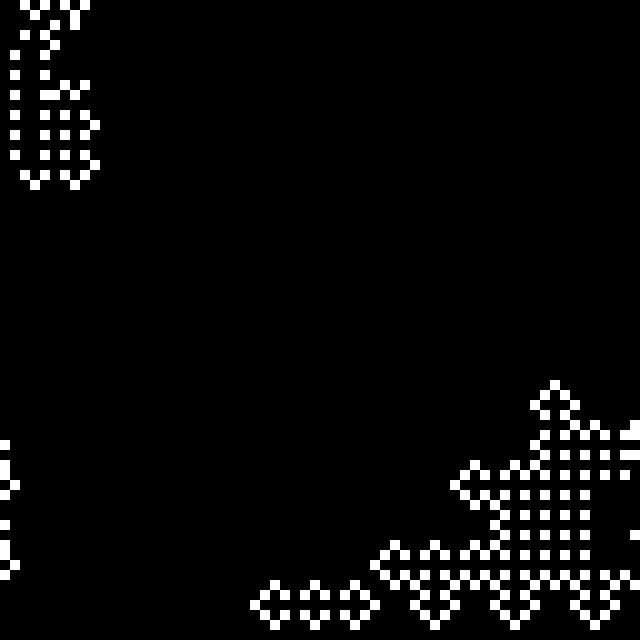
\includegraphics[width=\linewidth]{images/64x64_2_1.png}
\captionof{figure}{64x64}
\end{Figure}


%column2
\begin{Figure}
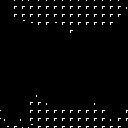
\includegraphics[width=\linewidth]{images/128x128_2.png}
\captionof{figure}{128x128}
\end{Figure}

\begin{Figure}
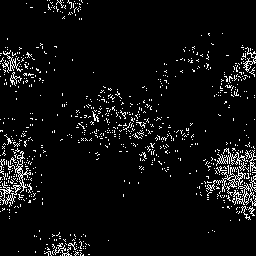
\includegraphics[width=\linewidth]{images/256x256_2.png}
\captionof{figure}{256x256}
\end{Figure}


%column3
\begin{Figure}
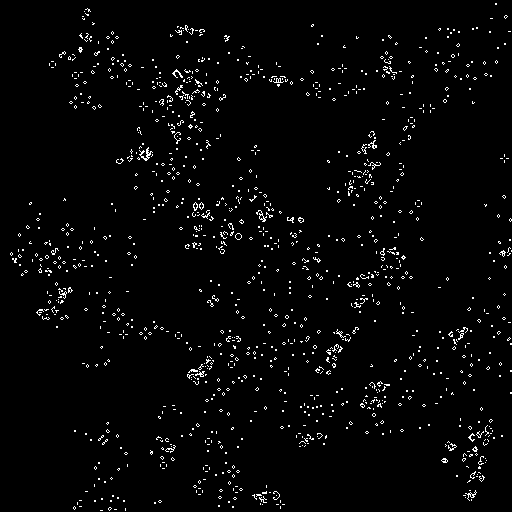
\includegraphics[width=\linewidth]{images/512x512_2.png}
\captionof{figure}{512x512}
\end{Figure}

\end{multicols}

\pagebreak
\section{Critical Analysis}
Through testing, it was determined that the additional time complexity of packing and unpacking meant that the



\bibliographystyle{unsrt}
\bibliography{}
\end{document}
